\section*{\bfseries\large\MakeUppercase{Appendix A}} \label{A}

\begin{center}
    \centering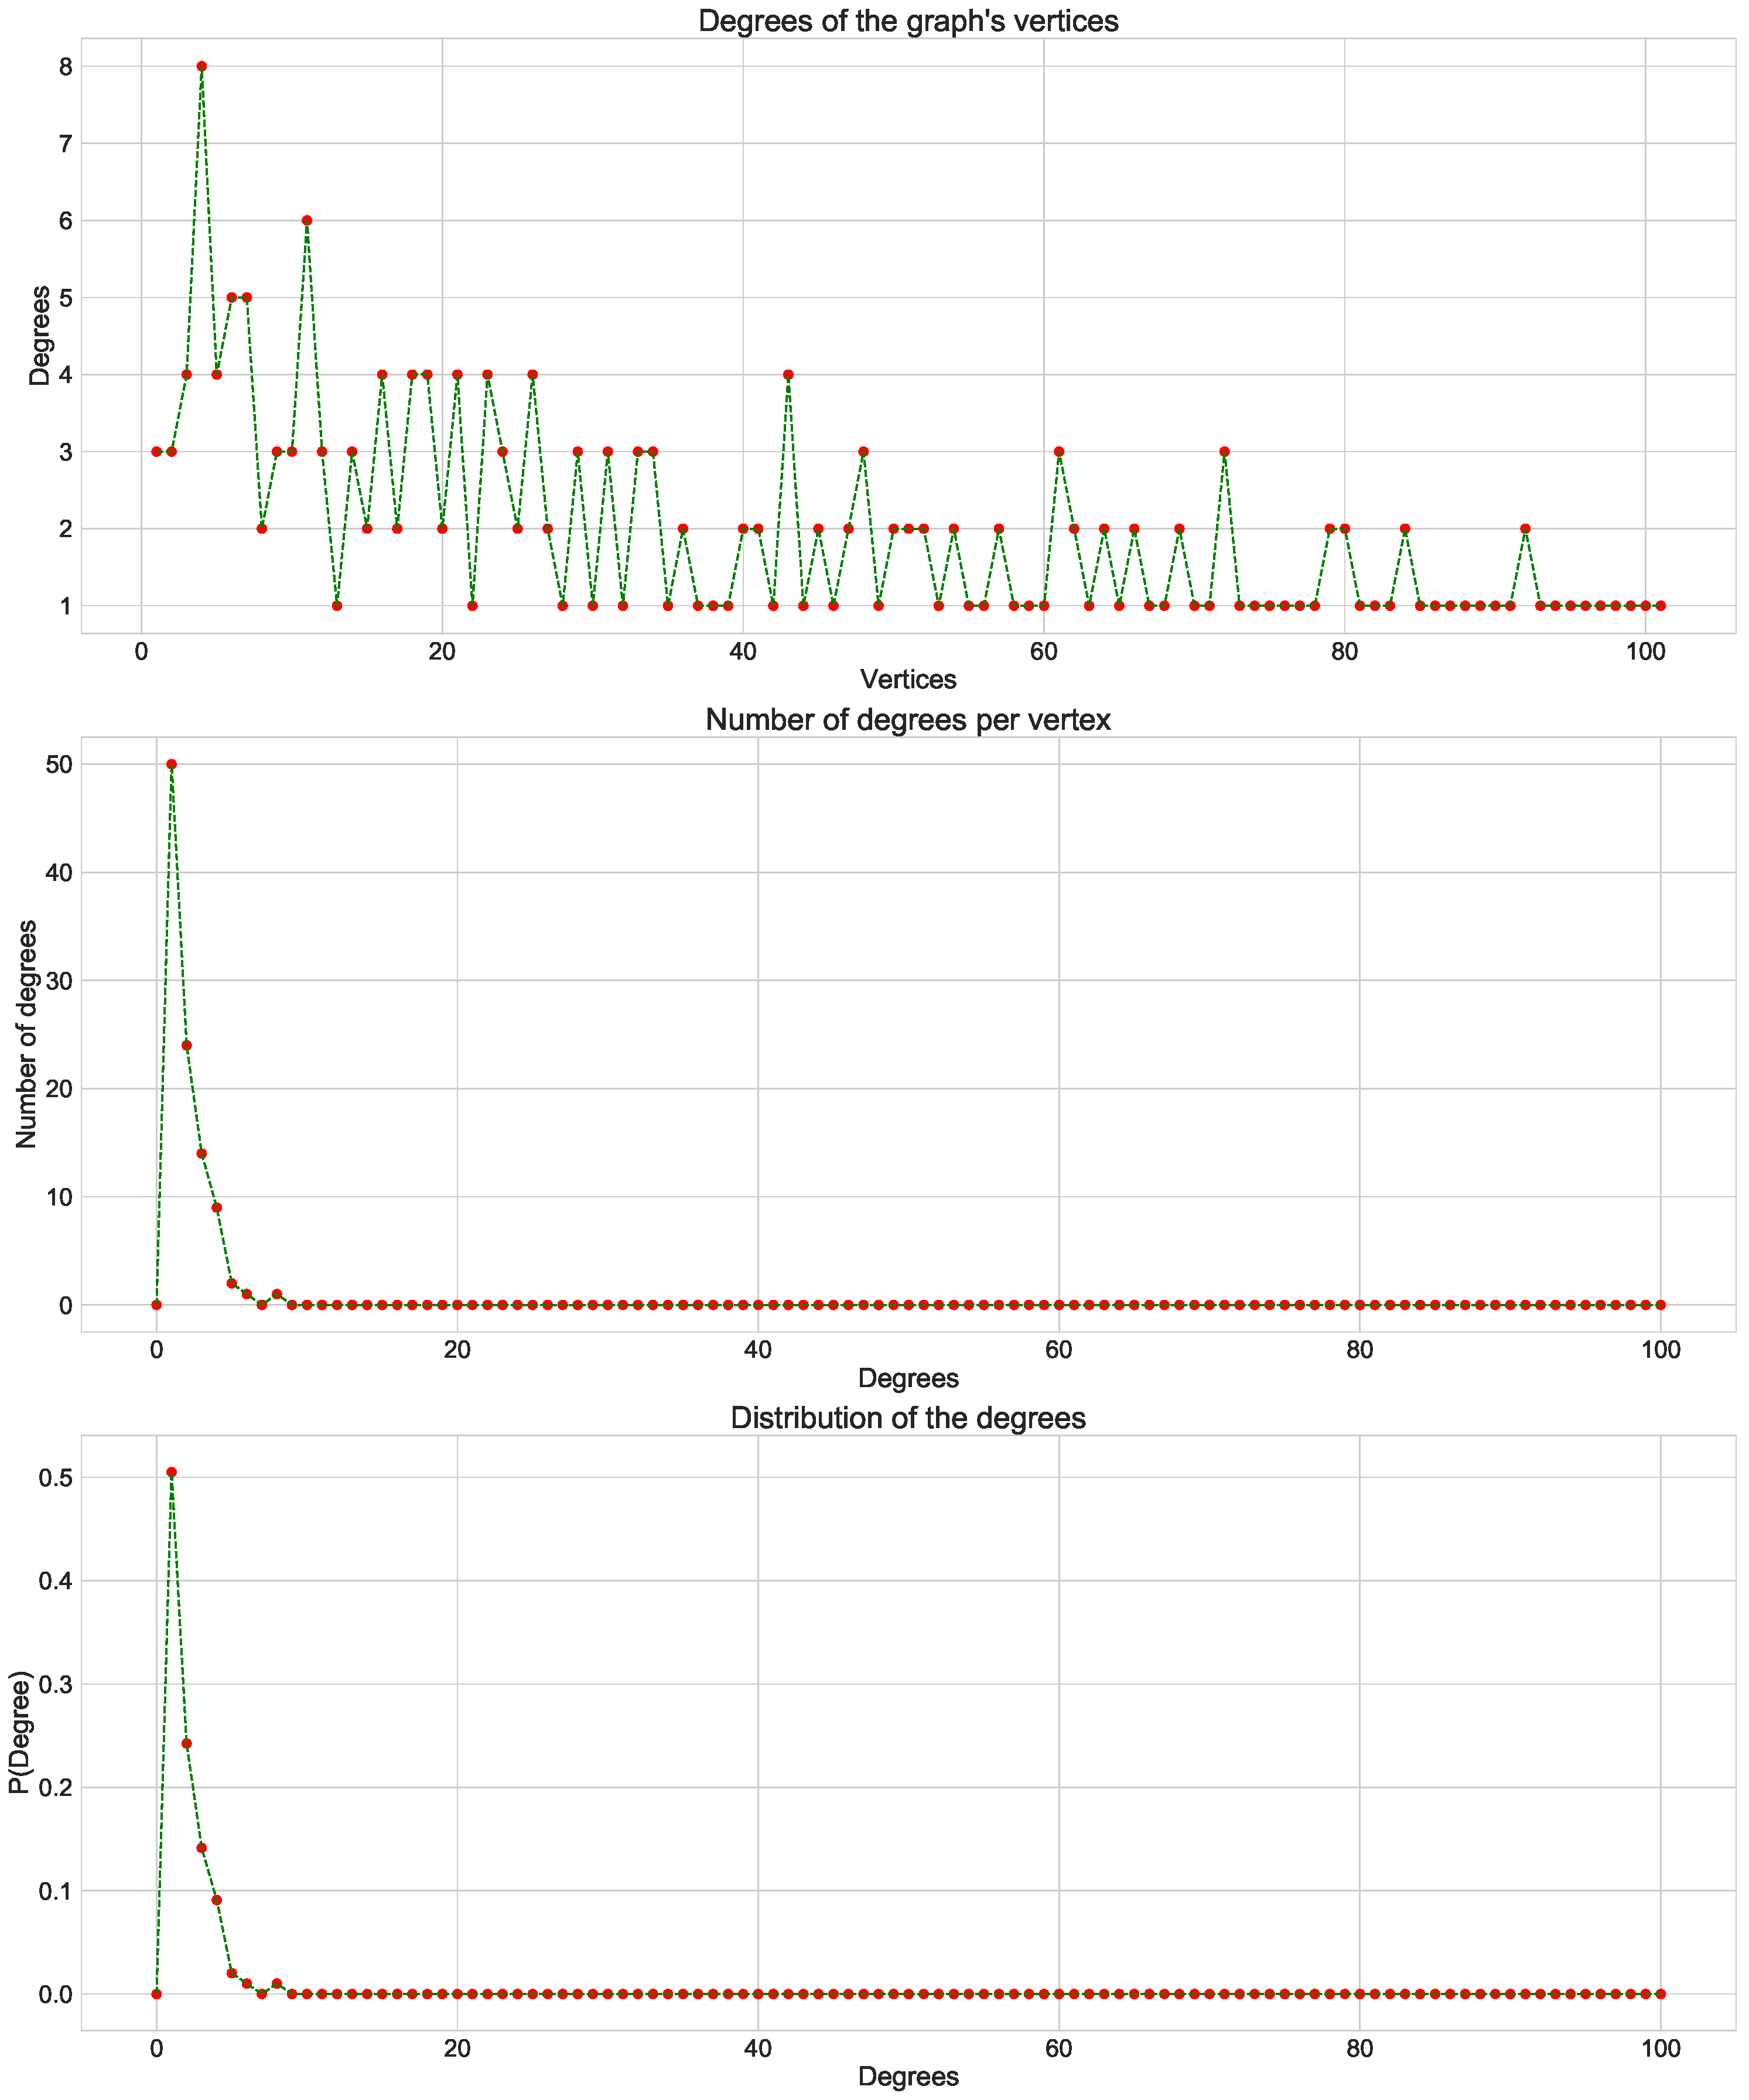
\includegraphics[width=0.9\textwidth]{images/rrt.pdf}
    \captionof{figure}{A \rrt $E=100$ élre\\Fent: Az egyes csúcsok fokszáma\\Középen: Adott fokszámú csúcsok darabszáma\\Lent: A csúcsok fokszámának eloszlása} \label{fig:1}
\end{center}
\newpage
\begin{center}
    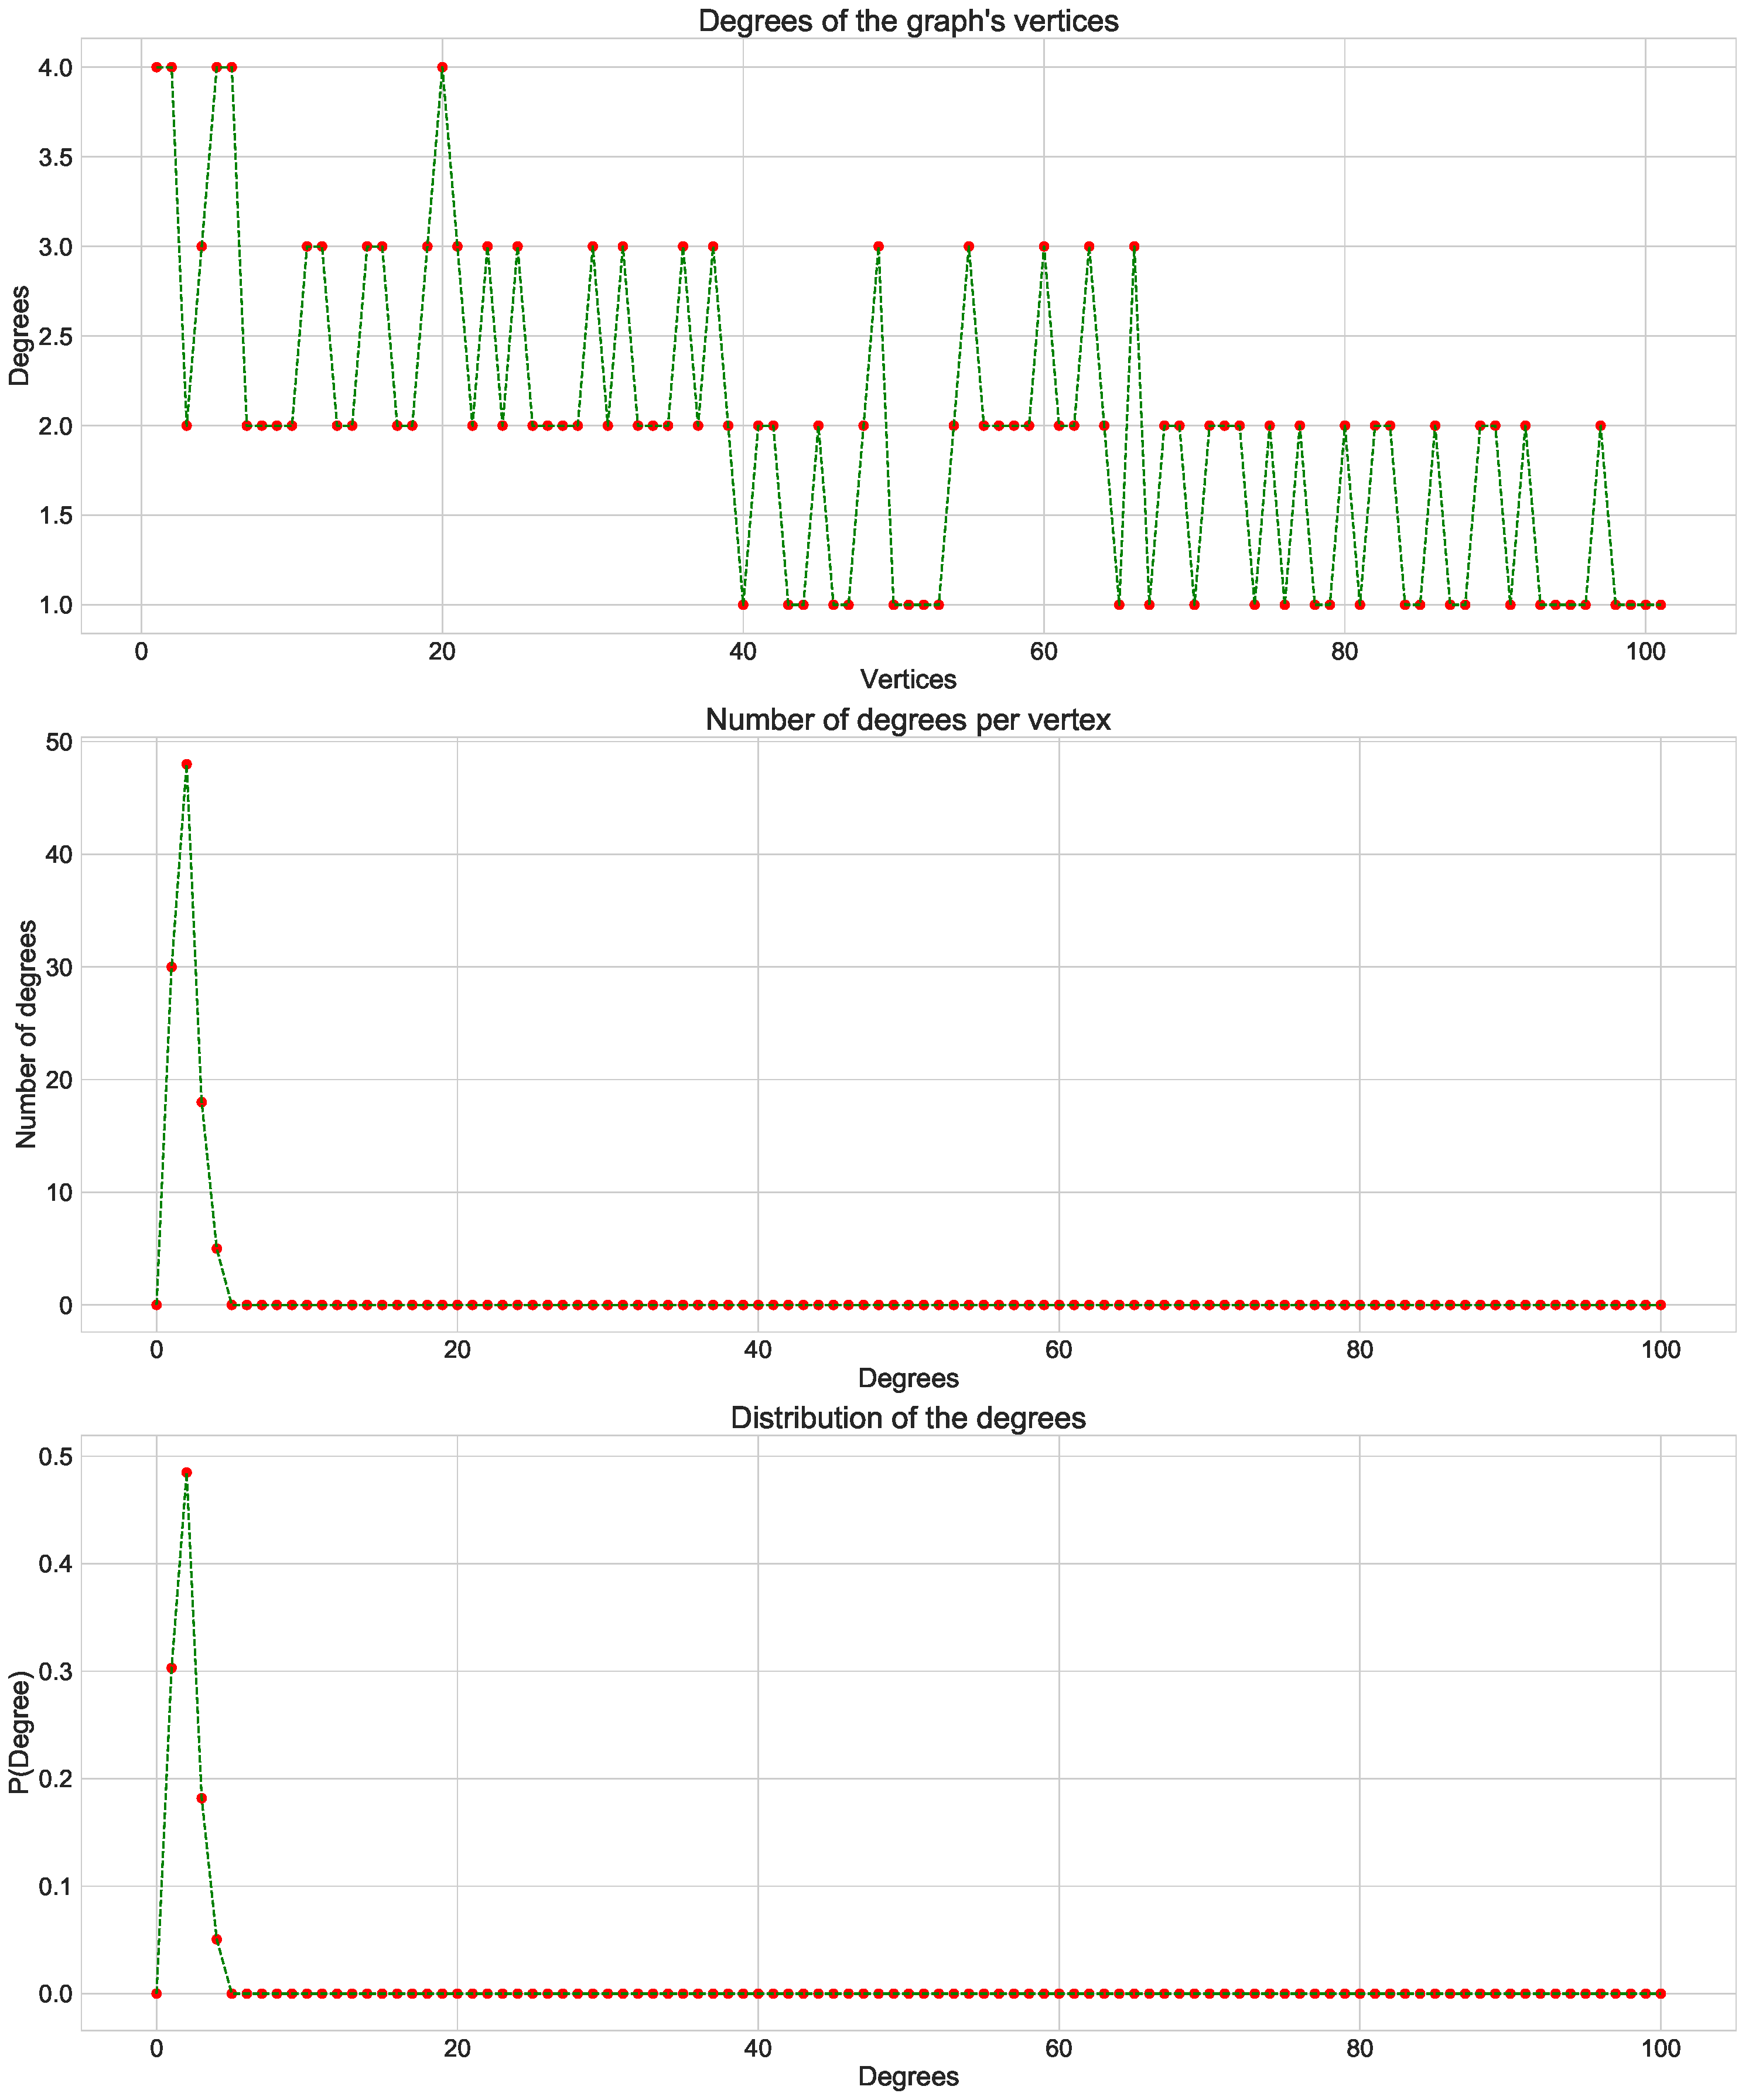
\includegraphics[width=0.95\textwidth]{images/apm.pdf}
    \captionof{figure}{Az \apm $E=100$ élre\\Fent: Az egyes csúcsok fokszáma\\Középen: Adott fokszámú csúcsok darabszáma\\Lent: A csúcsok fokszámának eloszlása} \label{fig:2}
\end{center}
\newpage
\topskip0pt
\vspace*{\fill}
\begin{center}
    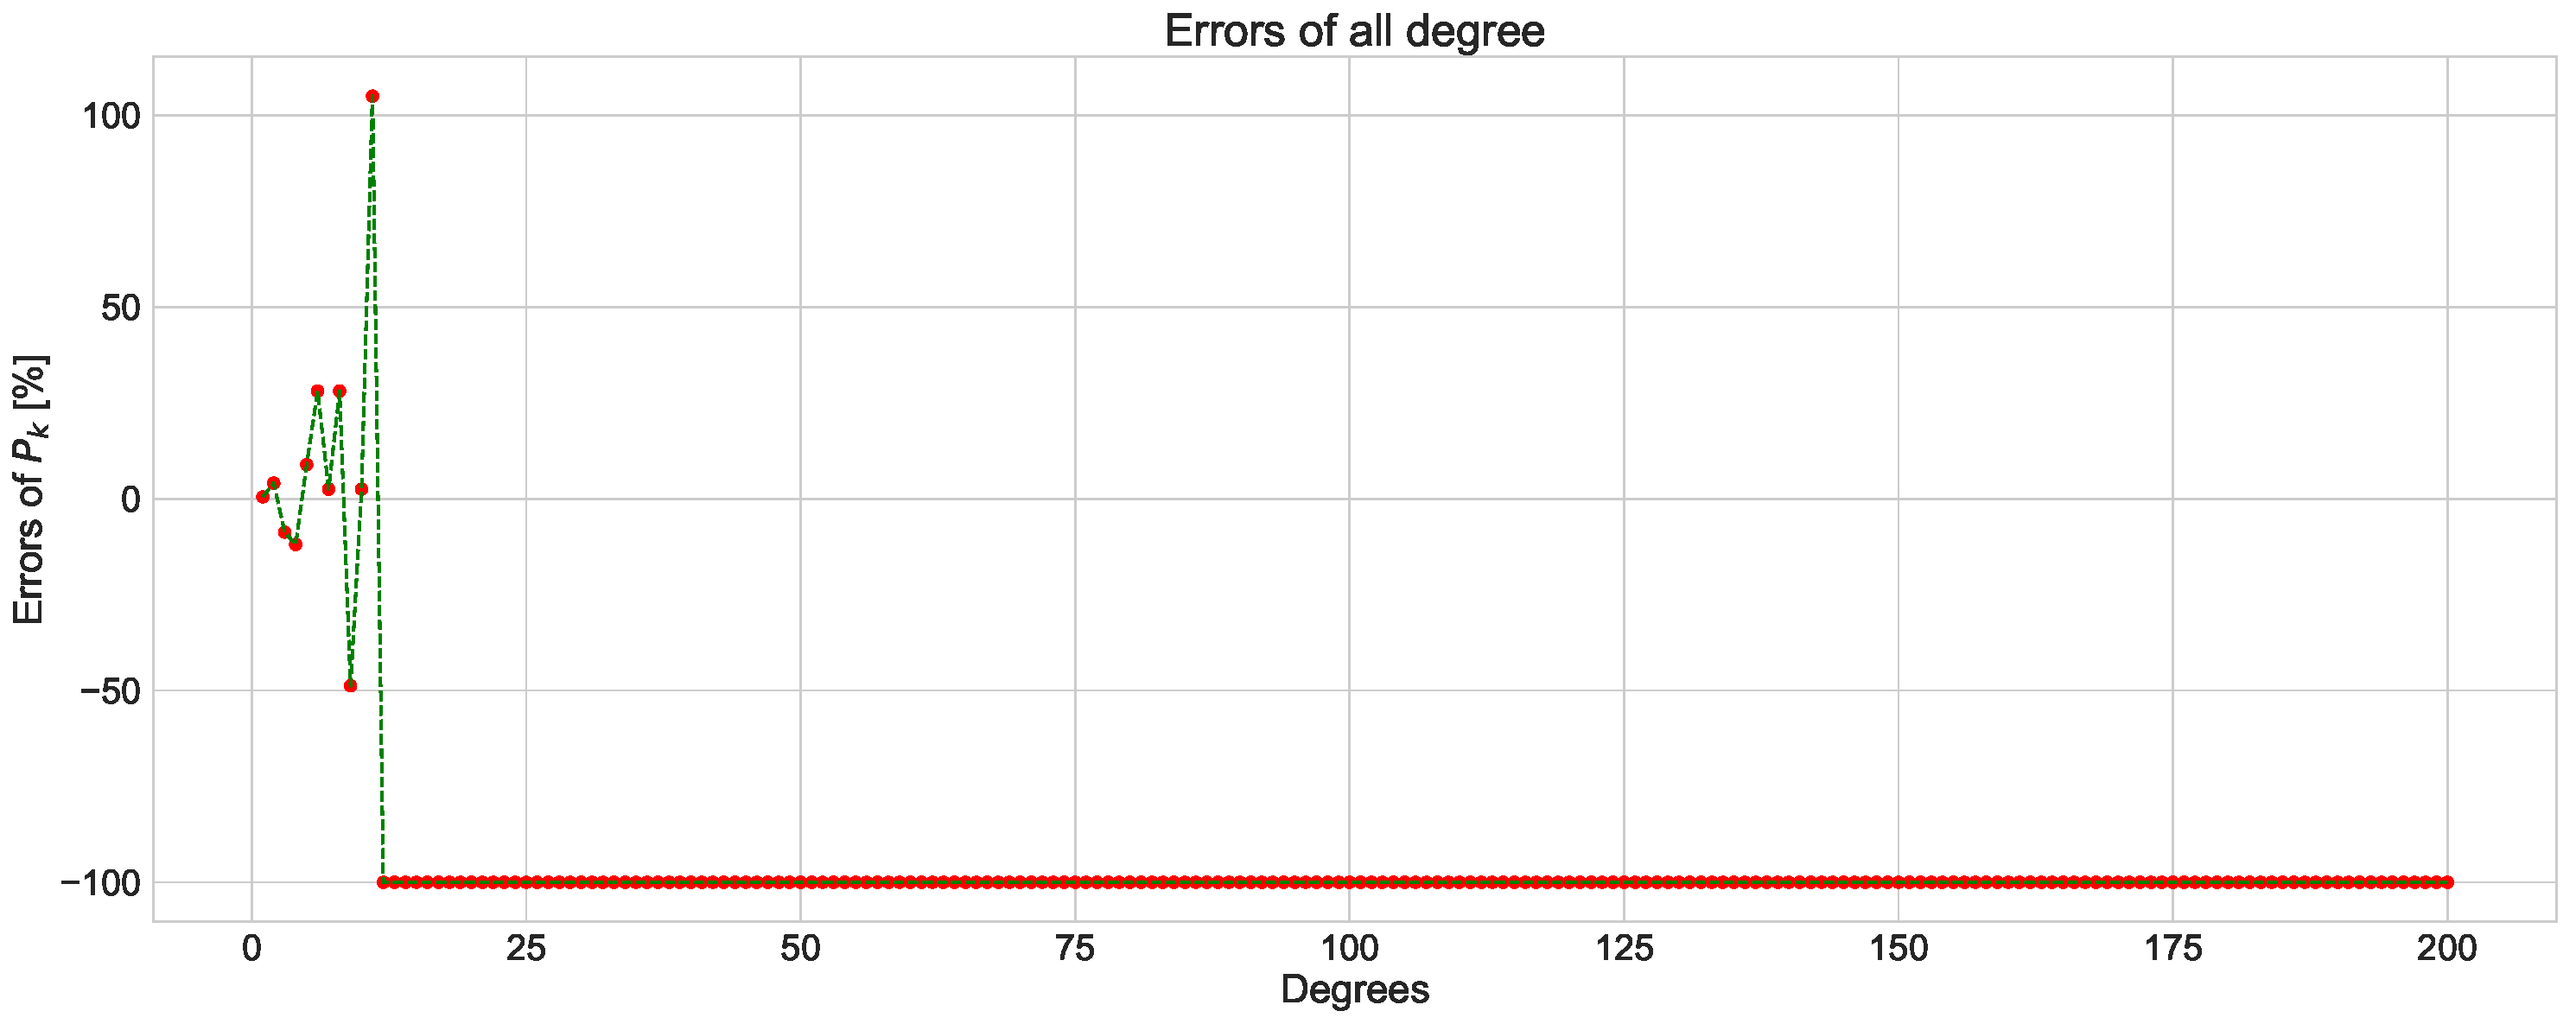
\includegraphics[width=\textwidth]{images/rrt_error_full.pdf}
    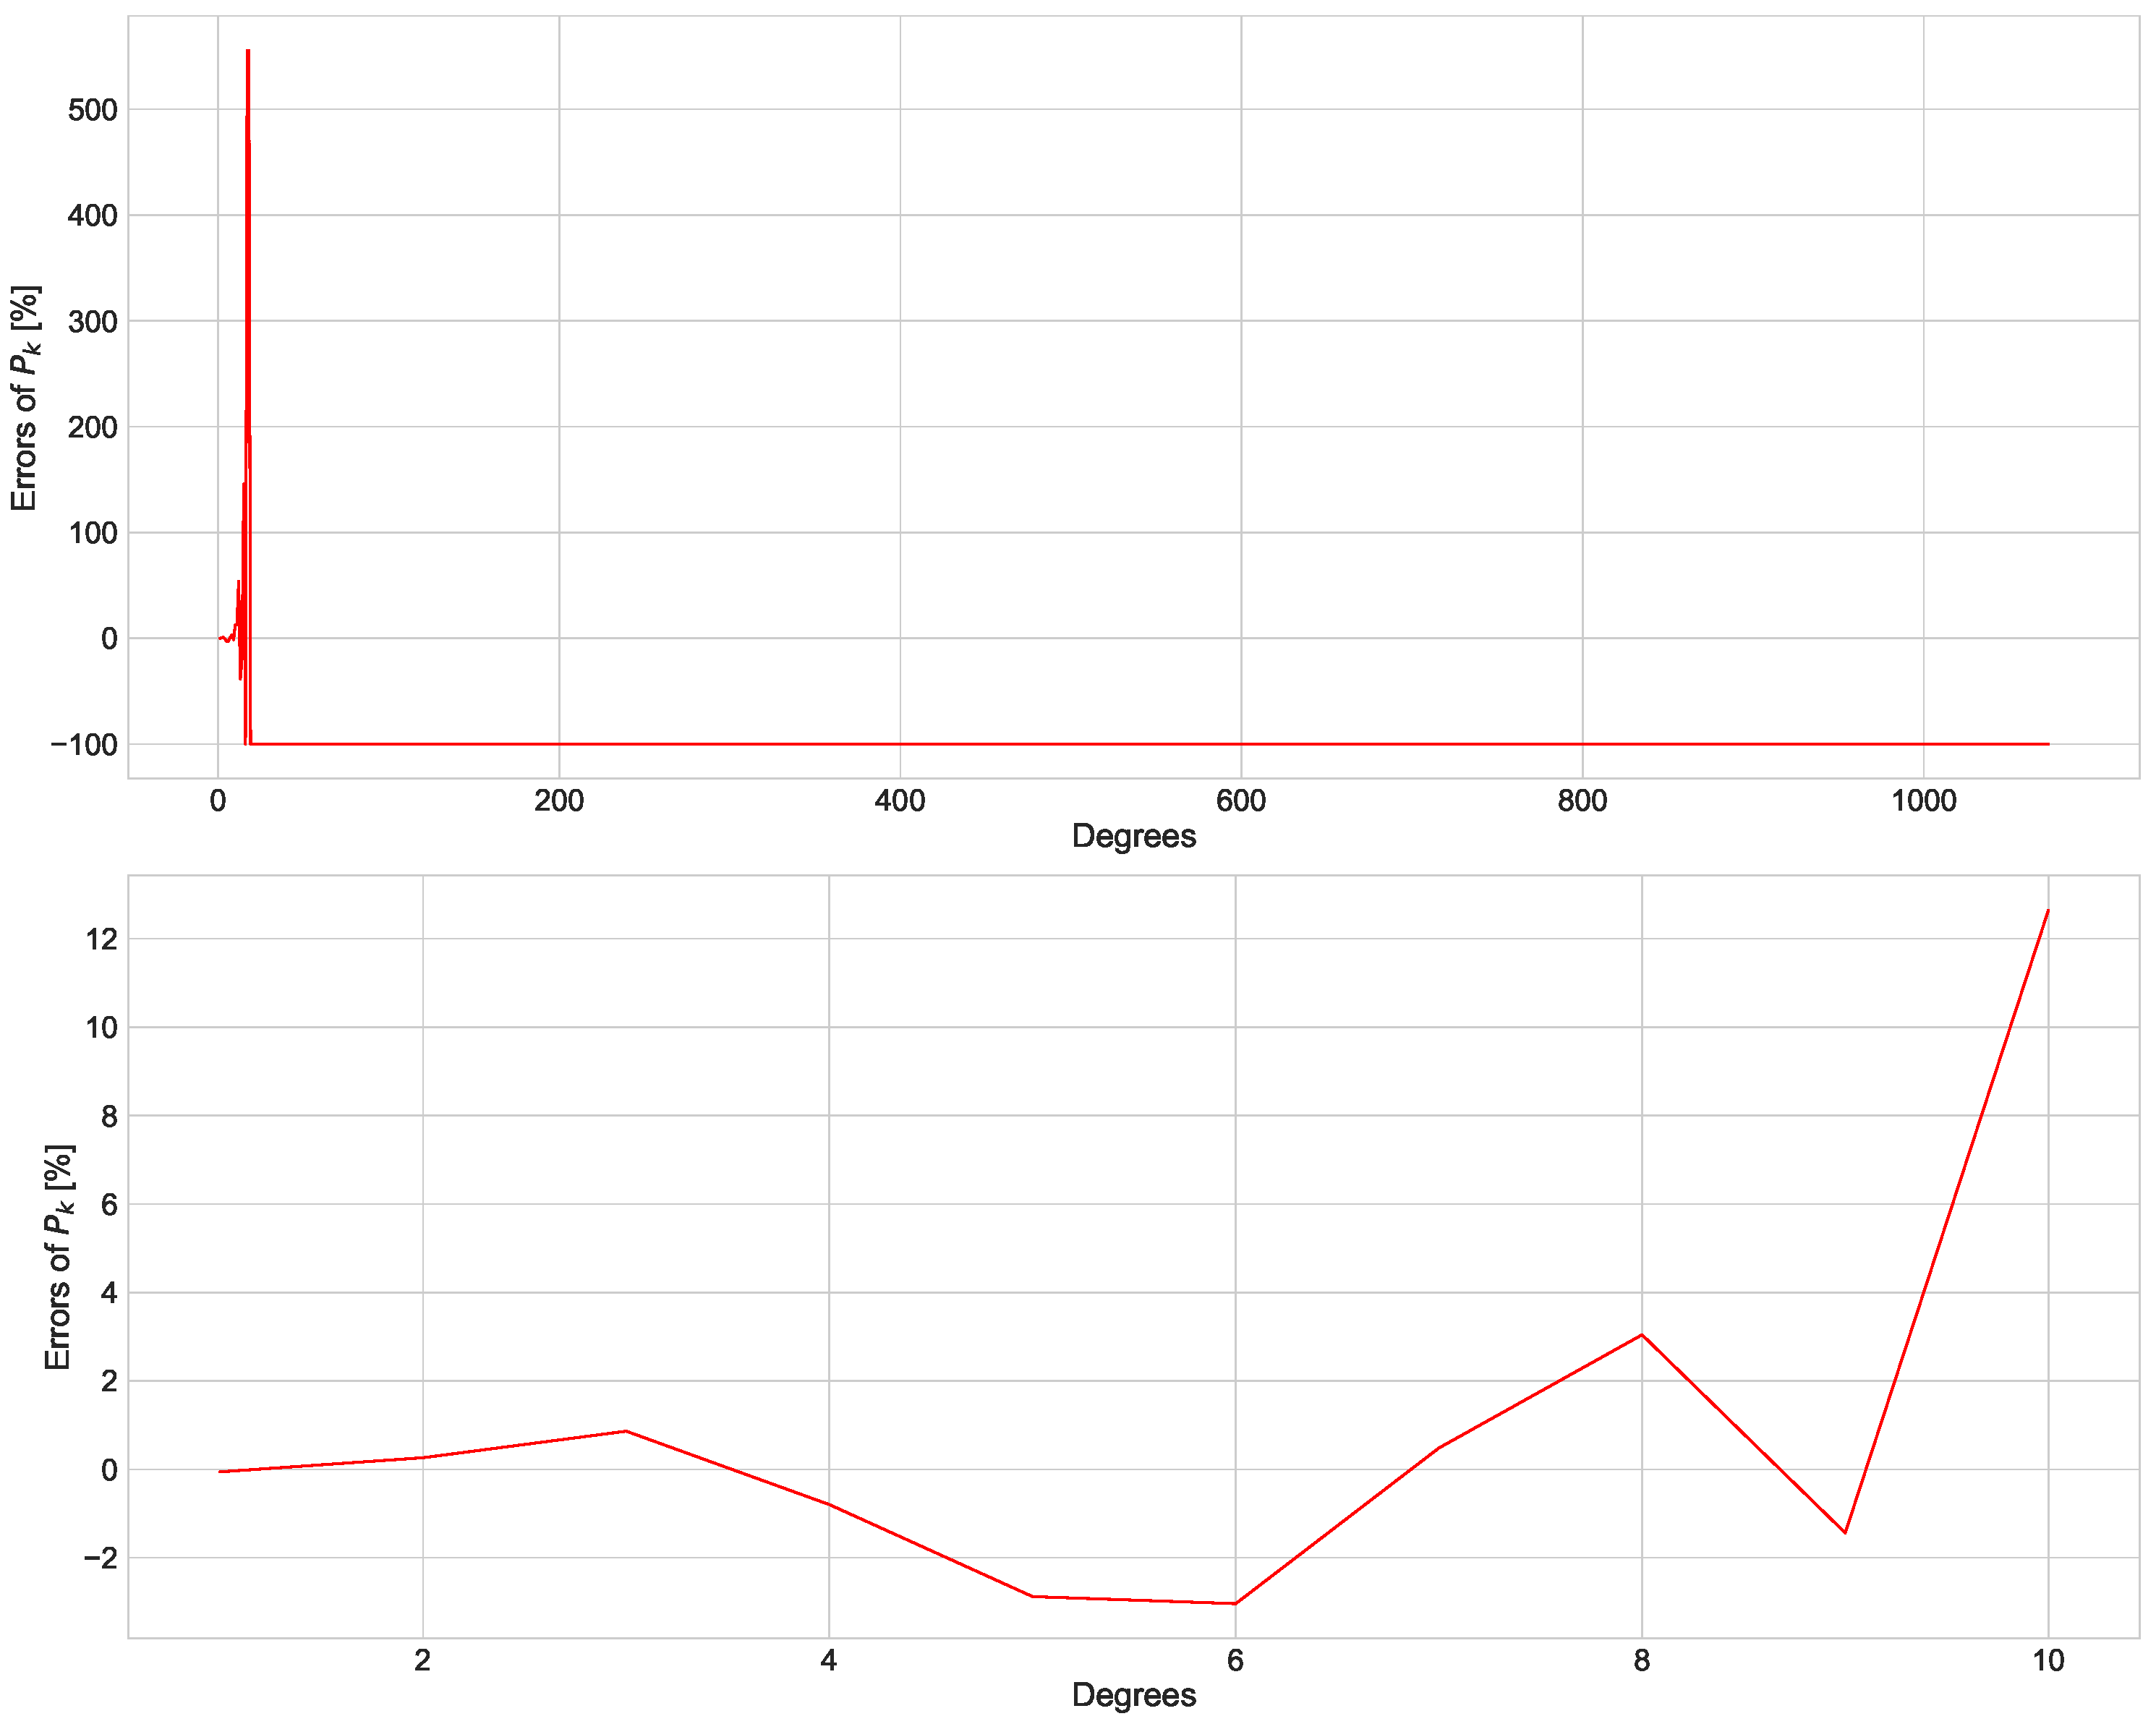
\includegraphics[width=\textwidth]{images/rrt_error.pdf}
    \captionof{figure}{A \rrt szimulációjának hibája a fokszámeloszlásra vonatkozóan\\Fent: A fokszámeloszlás teljes adatsorra vett százalékos eltérése. A $-100\%$-os értékek azt jelzik, hogy azokon a pontokon a szimuláció $k=0$-t adott eredményül, azonban az elméleti görbe egy exponenciális lecsengő függvény. Emiatt itt az eltérés az elméleti érték $100\%$-a.\\Lent: A fokszámeloszlás csak első $10$ értékéhez tartozó hiba ábrázolása.} \label{fig:3}
\end{center}
\vspace*{\fill}
\newpage
\topskip0pt
\vspace*{\fill}
\begin{center}
    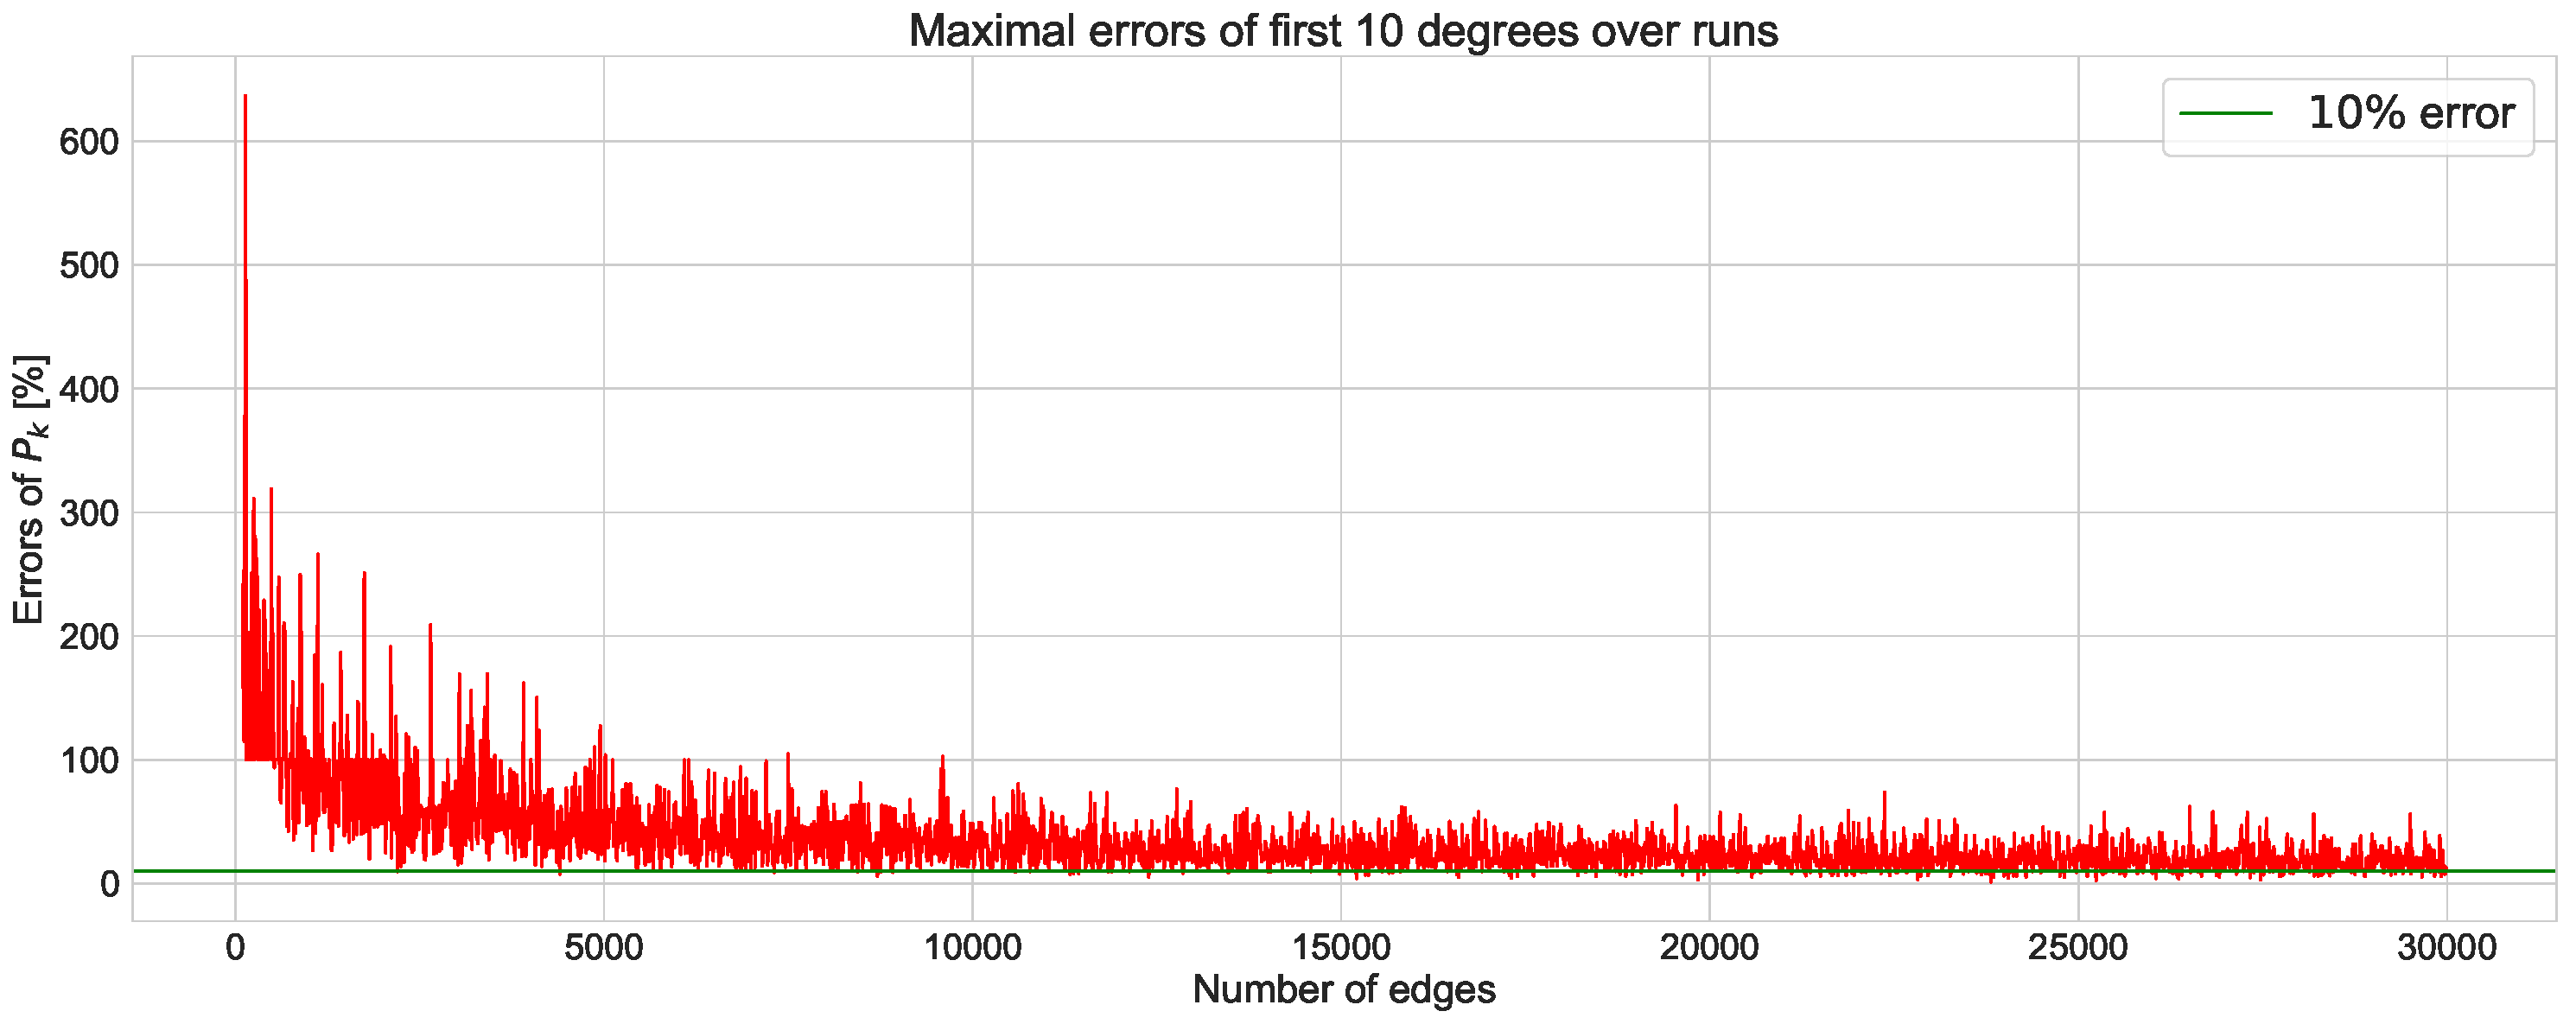
\includegraphics[width=\textwidth]{images/rrt_error_propag.pdf}
    \captionof{figure}{A \rrt különböző élszámokra mért $P_{k}$ élszámeloszlásának maximális eltérései az elméletileg számolt $P_{k} = e^{-k*\ln \left( 2 \right)}$ értéktől, az adatsor első $10$, legnagyobb fokszámú értékére. A görbe egyértelműen exponenciálisan csökkenő karakterisztikát mutat, mely a $10\%$-os értékhez propagál láthatólag. Mivel a futásidő már nagyon hosszú lett volna a későbbiekben, így nem tudtam a szimulációval nagyonn $E$ értékeket kipróbálni.} \label{fig:4}
\end{center}
\vspace*{\fill}
\newpage
\topskip0pt
\vspace*{\fill}
\begin{center}
    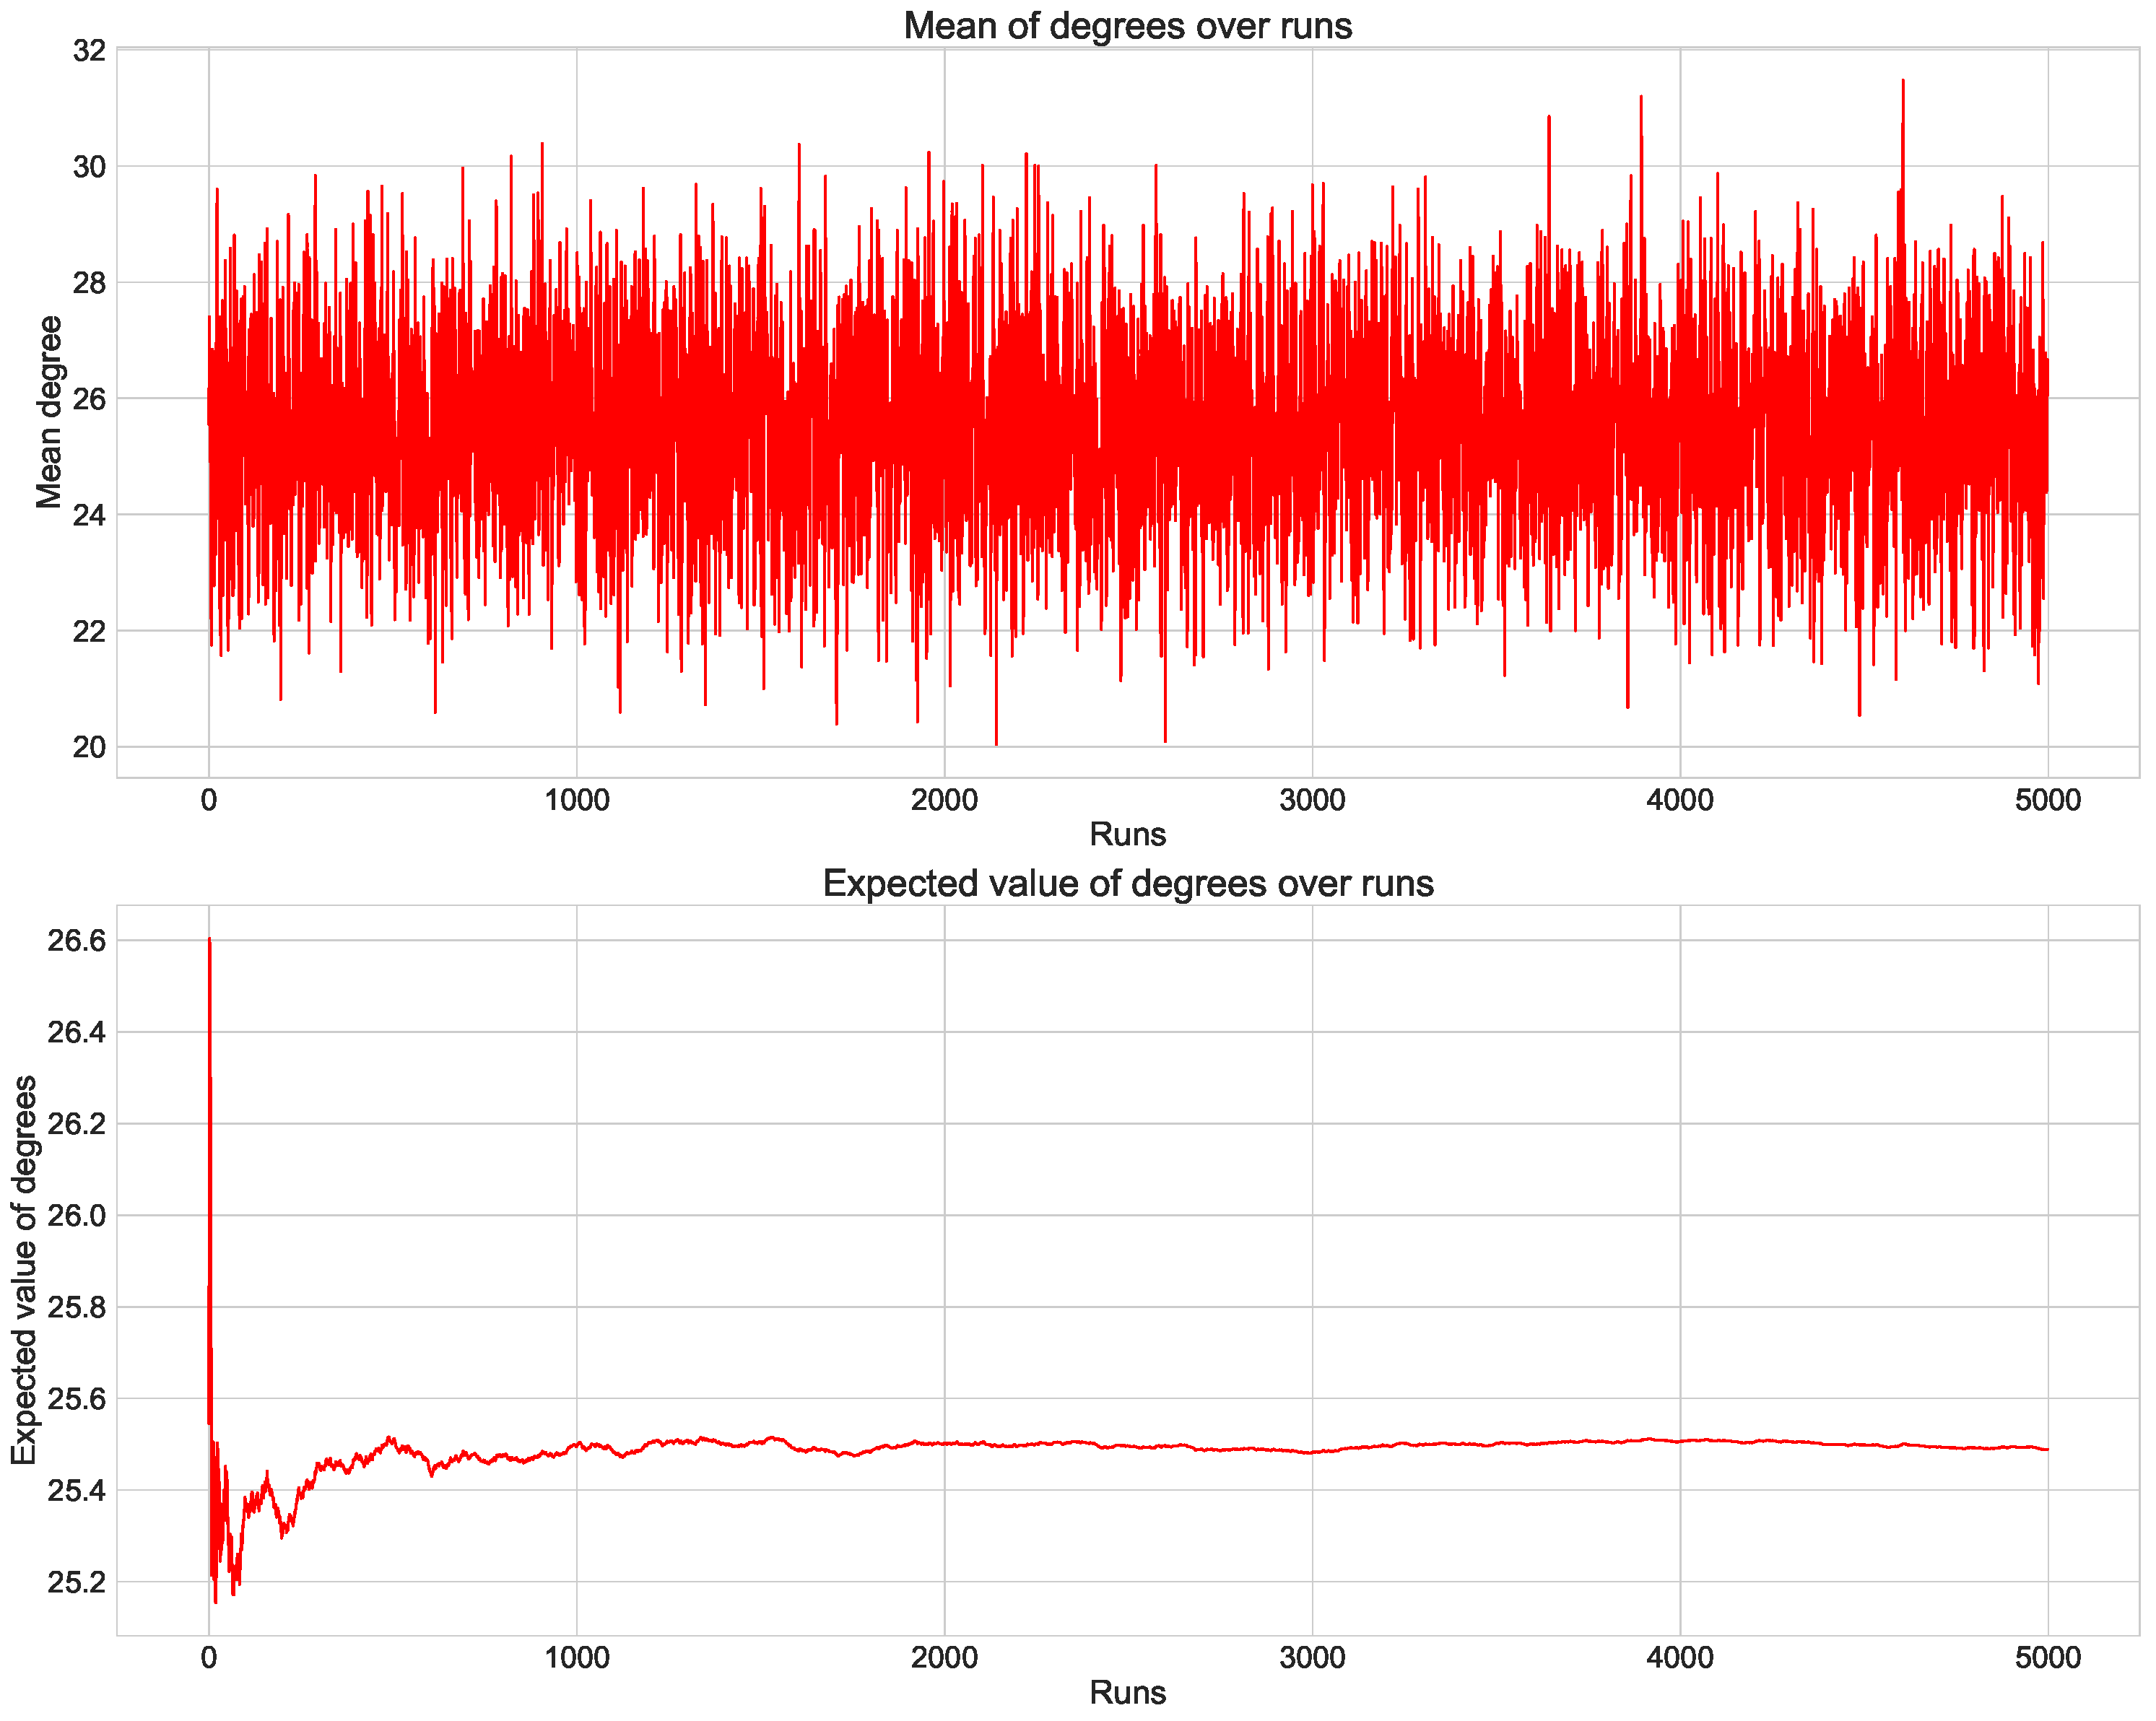
\includegraphics[width=\textwidth]{images/rrt_mean.pdf}
    \captionof{figure}{A \rrt különböző élszámokra mért átlagos fokszáma.\\A szimuláció $E=100$ és $E=5000$ élszámértékek között futott.} \label{fig:5}
\end{center}
\begin{center}
    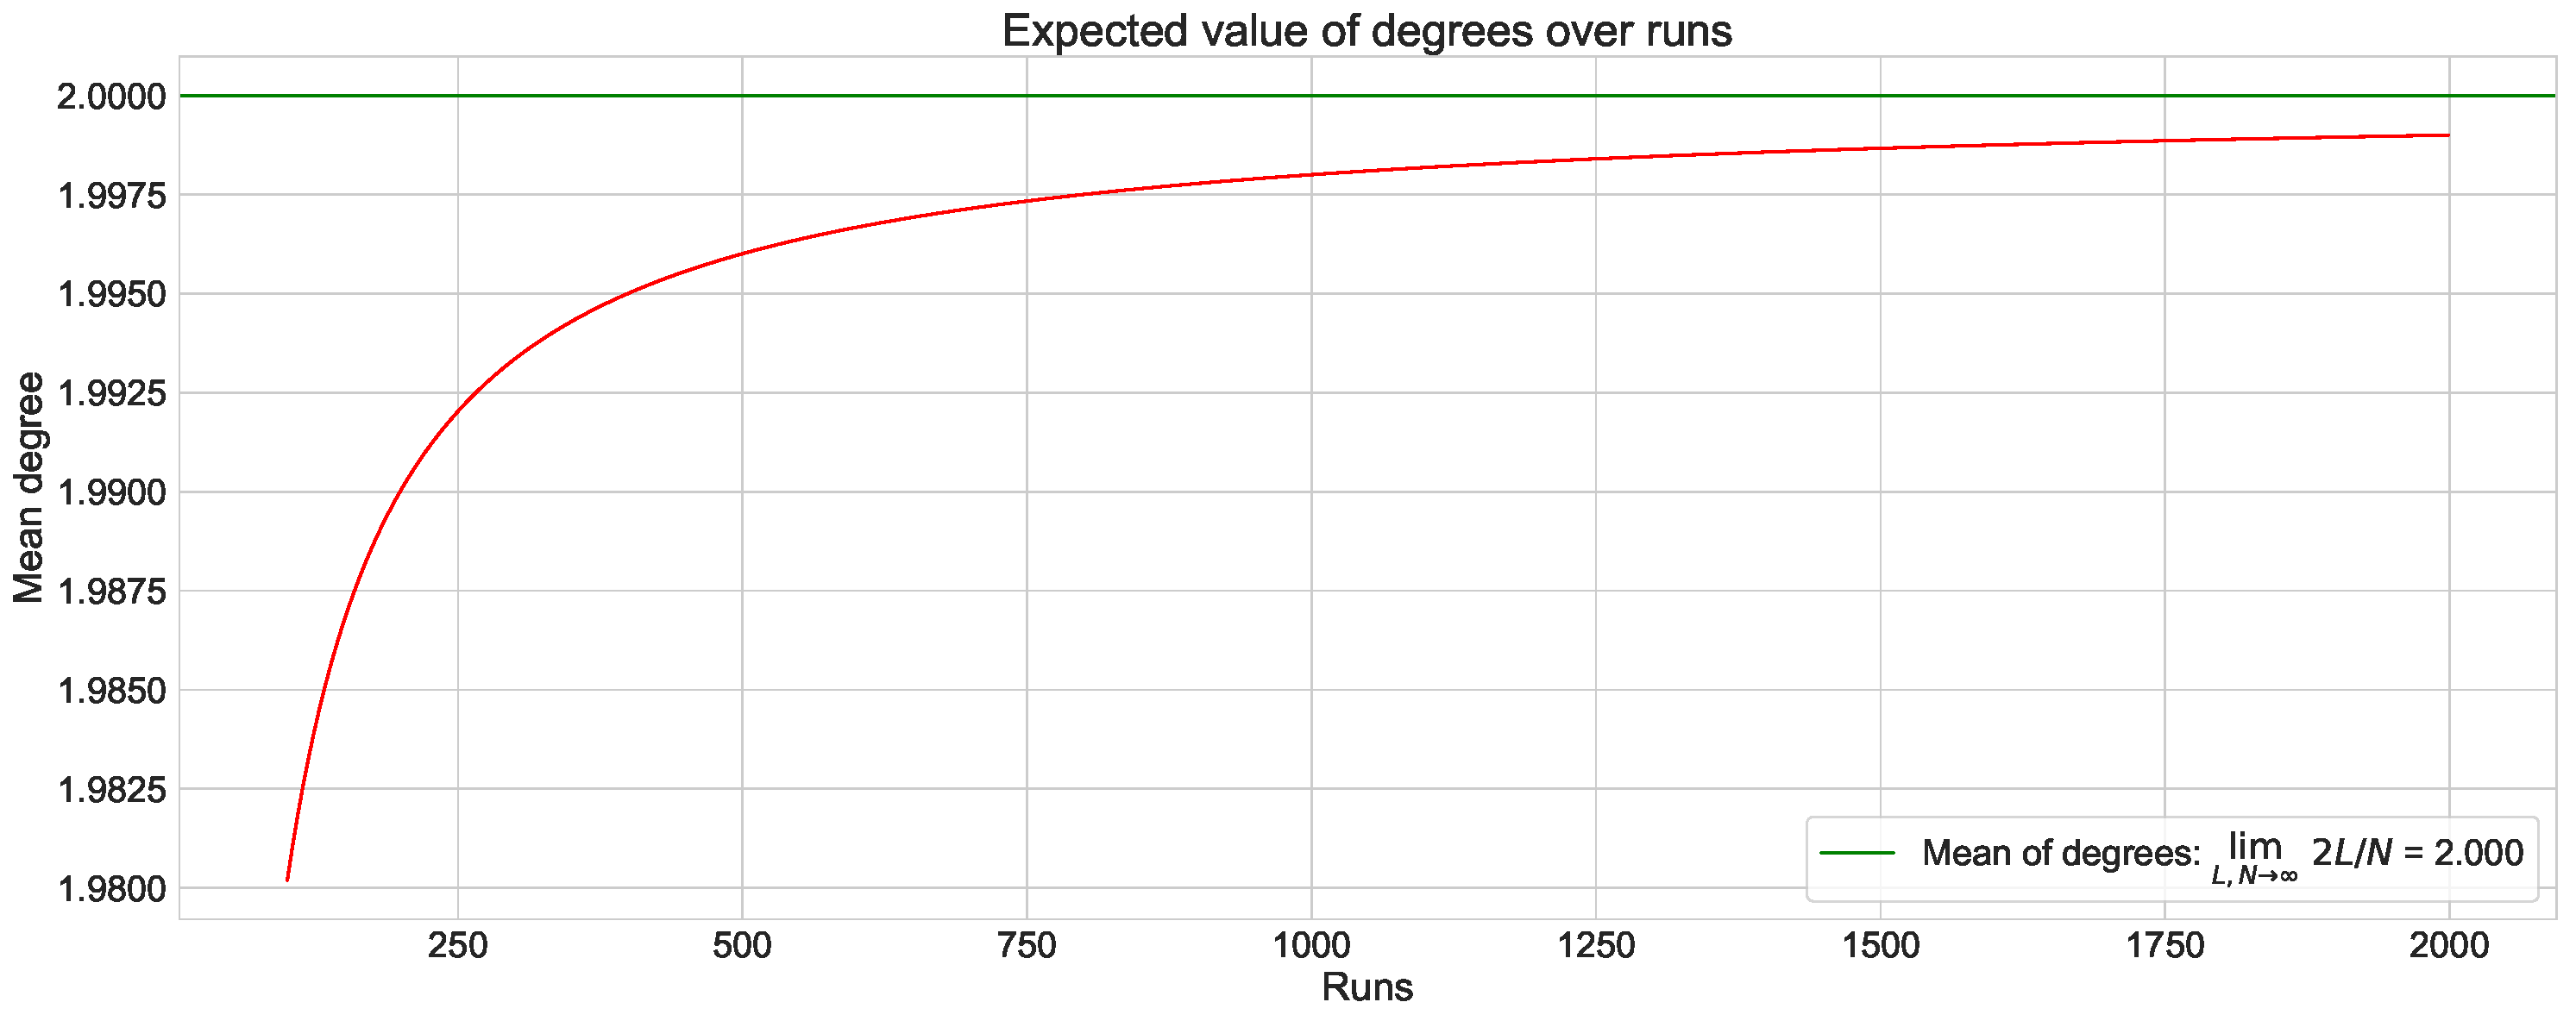
\includegraphics[width=\textwidth]{images/apm_mean.pdf}
    \captionof{figure}{Az \apm különböző élszámokra mért átlagos fokszáma.\\A szimuláció $E=100$ és $E=200$ élszámértékek között futott\protect\footnotemark.} \label{fig:6}
\end{center}
\vspace*{\fill}
\footnotetext{A két ábra megtévesztőnek tűnhet elsőre. Az átlagos fokszámok mind a \rrt, mint az \apm esetén hasonlóan alakultak, azonban az \apm esetén a futásidő jóval hosszabb volt. Emiatt az élszámok csupán szűk intervallumában tudtam lemérni az egyes átlagos értékeket. Hogy a hasonlóságot szemléltethessem, az \apm ábráján a \rrt görbéjét is ábrázoltam, az előbbivel azonos intervallumban. Ezt az ábrán látható jelmagyarázatban jelöltem is.}
\newpage
\topskip0pt
\vspace*{\fill}
\begin{center}
    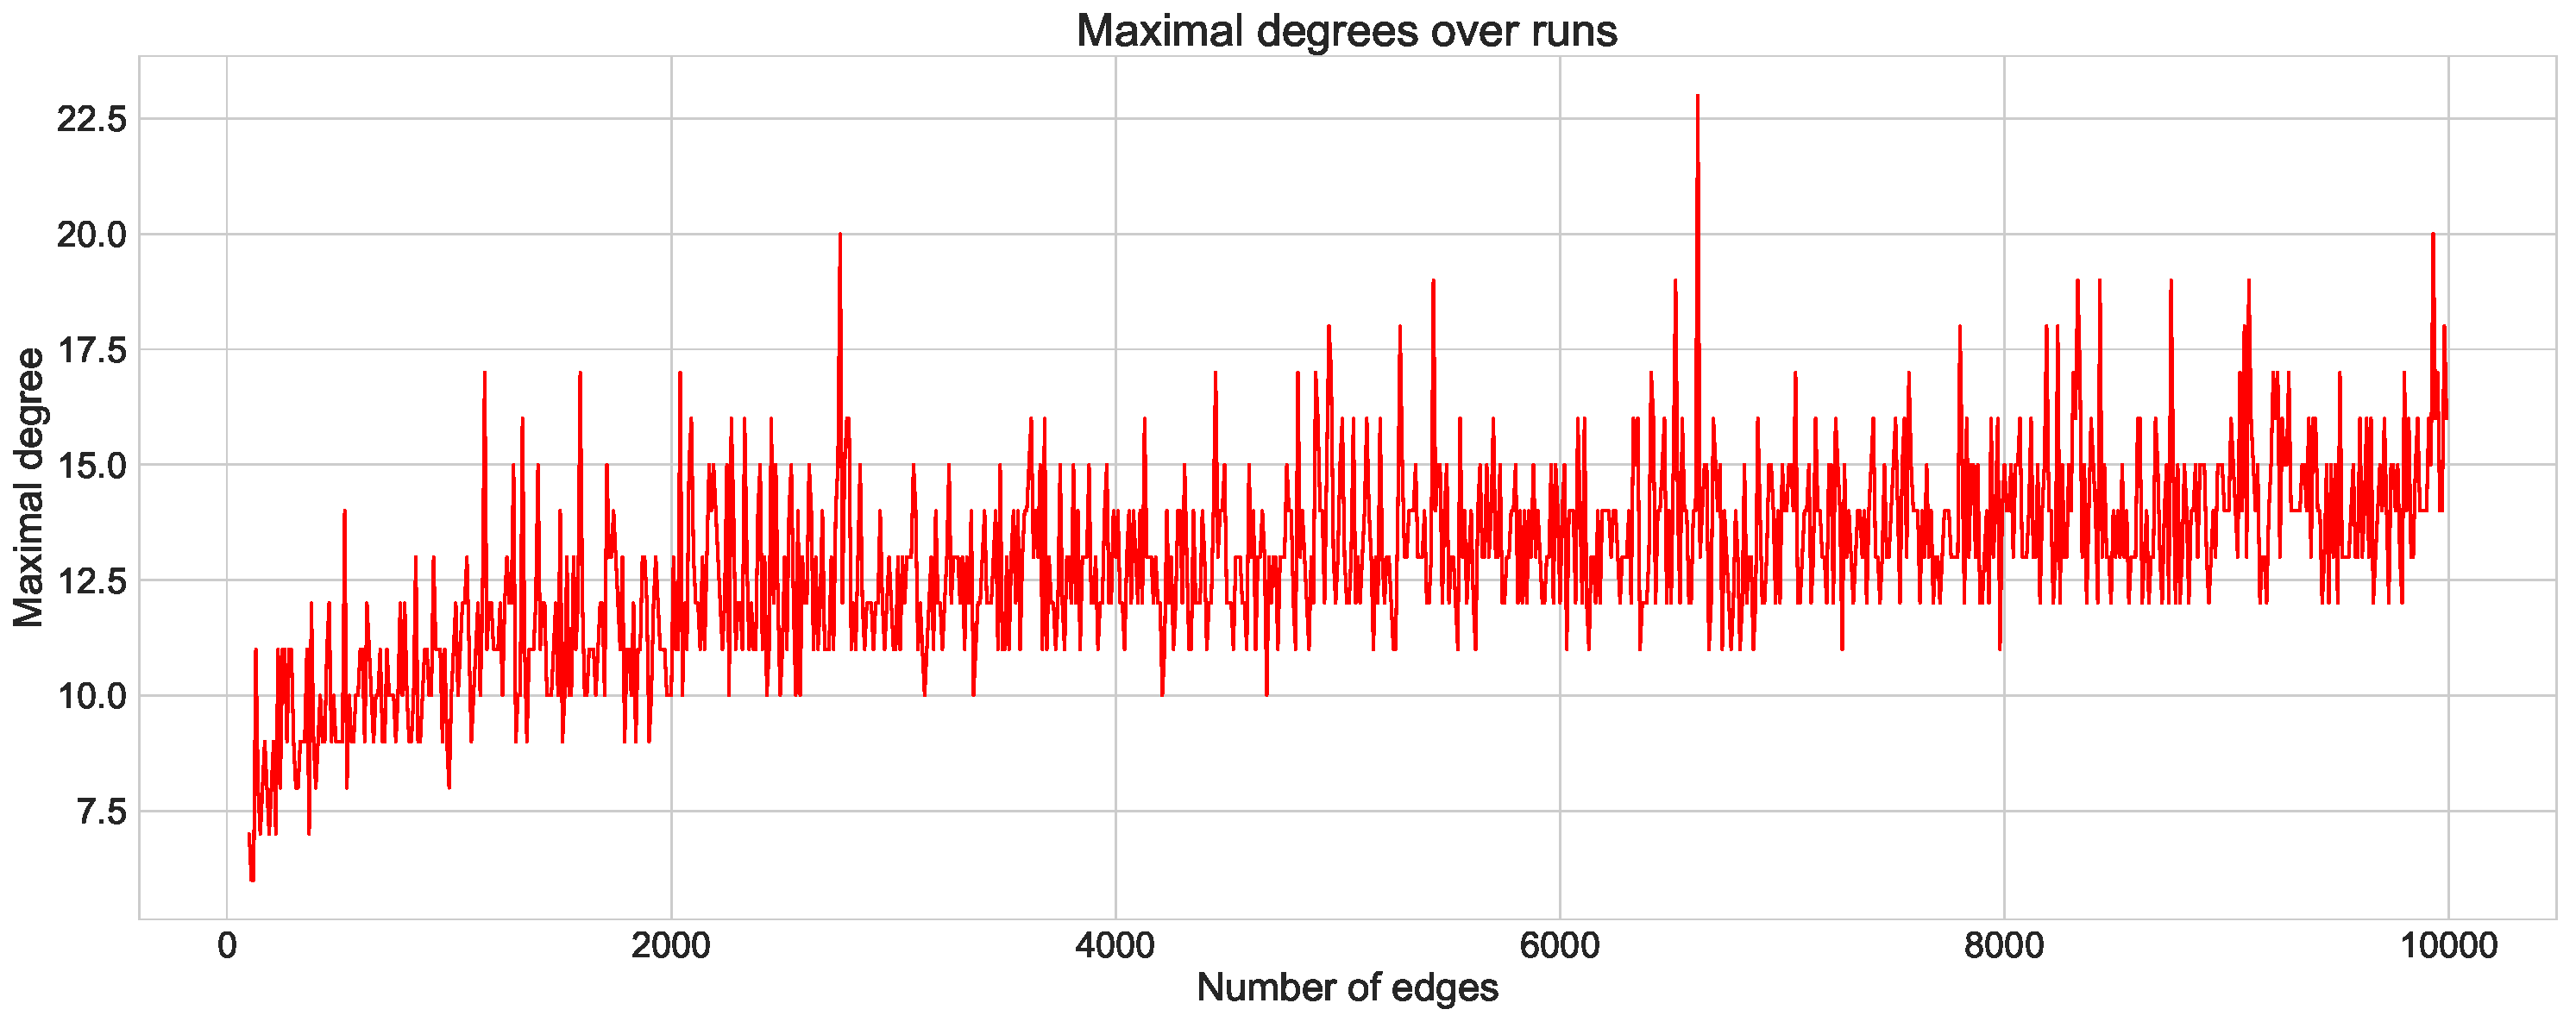
\includegraphics[width=\textwidth]{images/rrt_maxdegrees.pdf}
    \captionof{figure}{A \rrt különböző $E$ élszámok esetén megjelenő maximális fokszáma.\\A szimuláció $E=100$ és $E=10000$ élszámértékek között futott.} \label{fig:7}
\end{center}
\begin{center}
    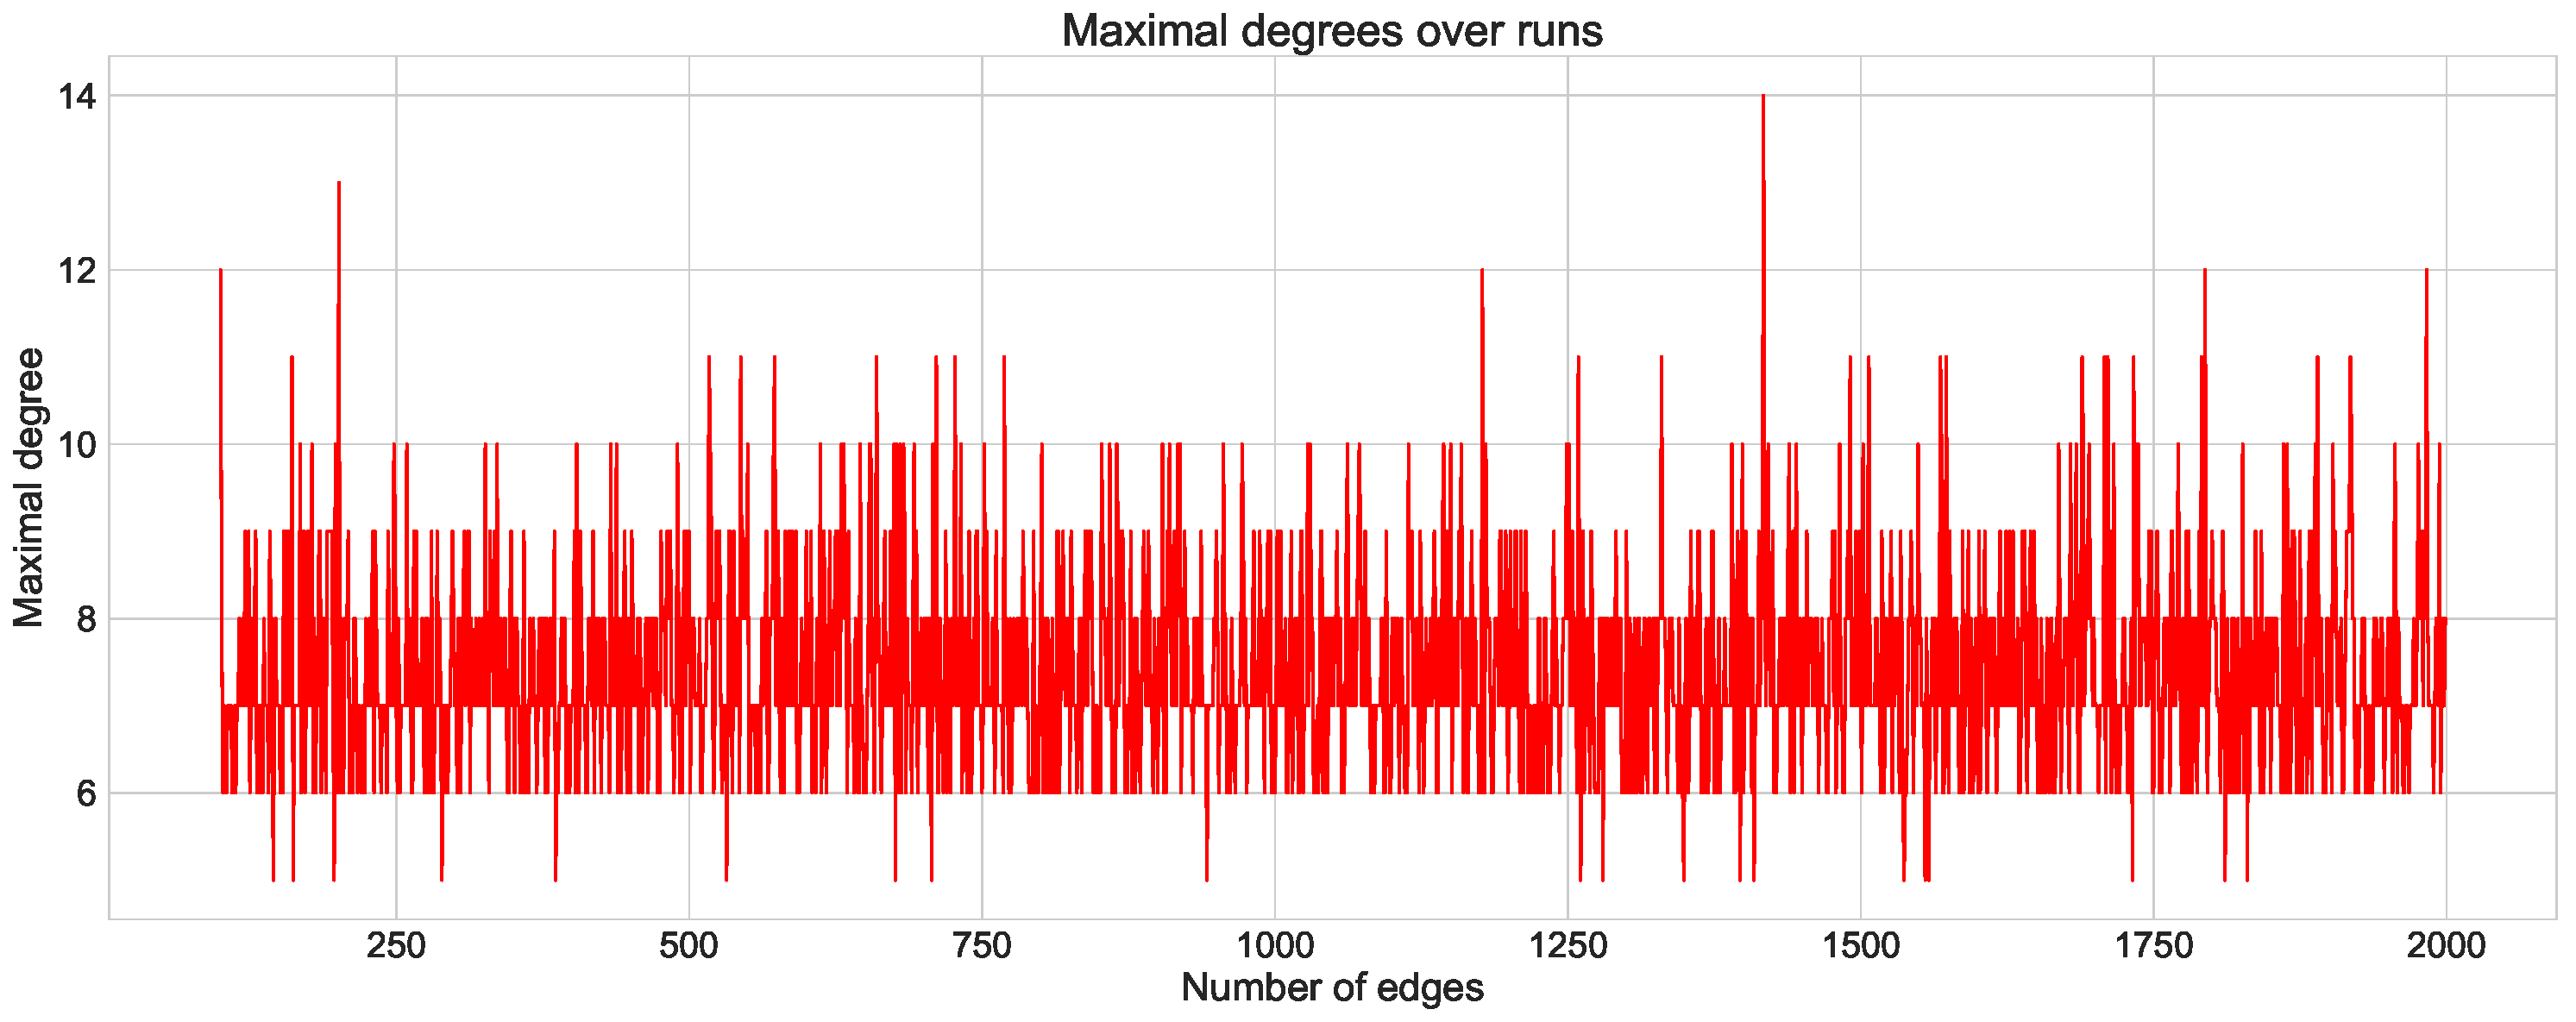
\includegraphics[width=\textwidth]{images/apm_maxdegrees.pdf}
    \captionof{figure}{Az \apm különböző $E$ élszámok esetén megjelenő maximális fokszáma.\\A szimuláció $E=100$ és $E=2000$ élszámértékek között futott.} \label{fig:8}
\end{center}
\vspace*{\fill}
\newpage
\topskip0pt
\vspace*{\fill}
\begin{center}
    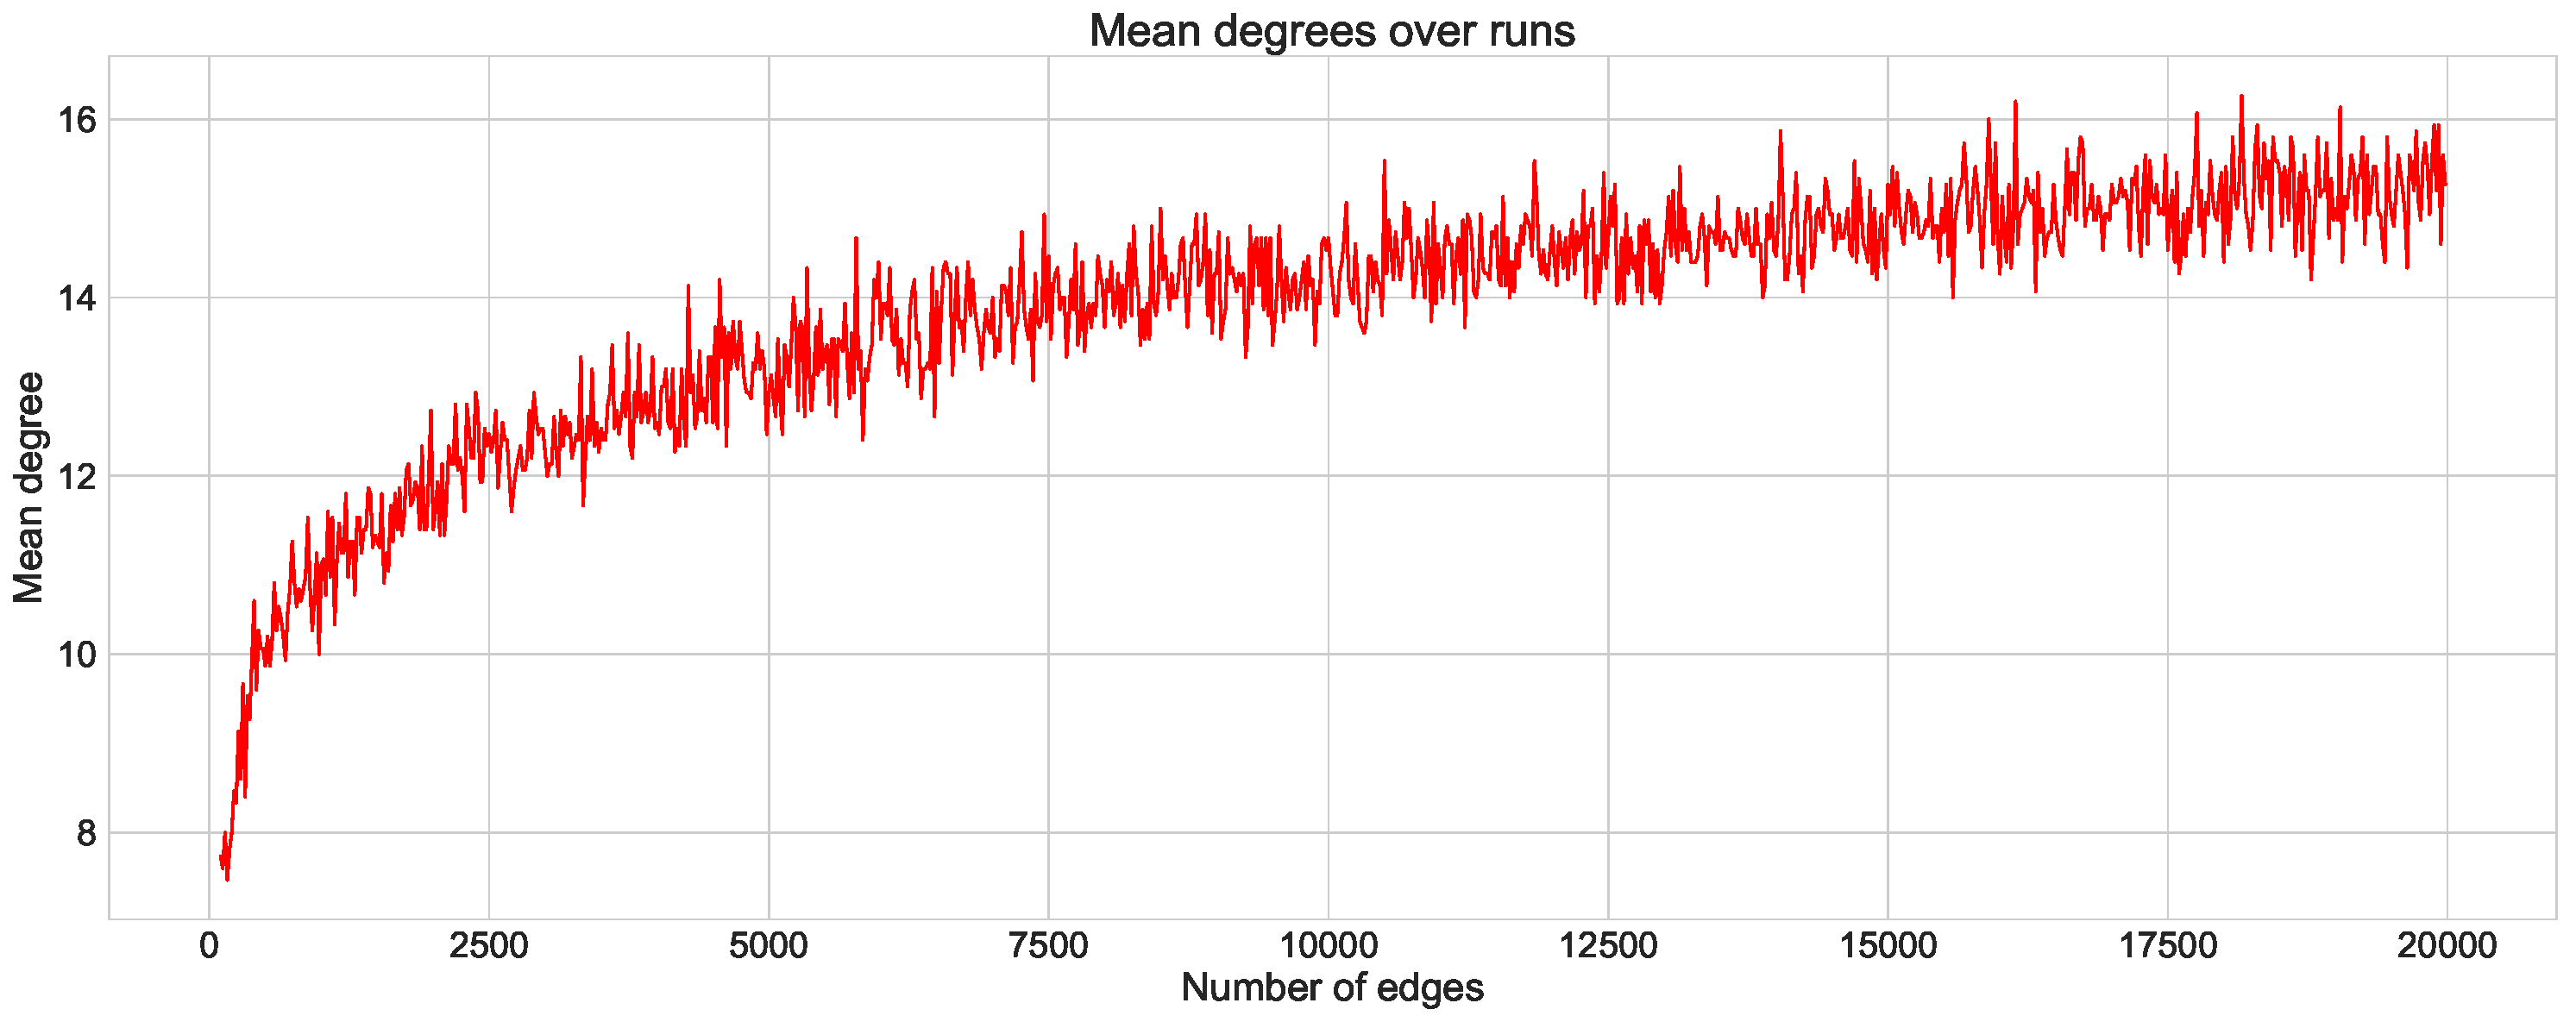
\includegraphics[width=\textwidth]{images/rrt_meandegrees.pdf}
    \captionof{figure}{A \rrt modell fokszámeloszlásának átlaga az $E$ élszám függvényében. Minden átlag $n=15$ db azonos élszámú futtatás eredményeiből lett számolva.} \label{fig:9}
\end{center}
\vspace*{\fill}